% This is an included file. See the master file for more information.
%
% This is an included file. See the master file for more information.
%

\chapter{Introduction}
\label{chap:introduction}
Extreme scale computers (such as proposed Exascale computers) contain
so many components that the aggregate mean-time-between-failure (MTBF)
is small
compared to the runtime of an application. Programming models (and
supporting compilers and runtime systems) must therefore support a
variety of features unique to these machines:
\begin{itemize}
\item The ability for a programmer to
express O(billion) concurrency in an application program.

\item The ability of a computation to make progress towards a useful
result even as components within the system fail.

\item The ability of a computation to dynamically adapt to a high
degree of variability in the performance and energy consumption of
system components to support efficient execution.

\item The ability to either hide overheads behind useful computation
or have overheads small enough to allow applications to exhibit strong
scaling across the entire exascale system.

\end{itemize}

There are a number of active research projects to develop runtime systems
for extreme scale computers. This specification describes one of
these research runtime systems: the \emph{Open Community Runtime} or \emph{OCR}.

The fundamental idea behind OCR is to consider a computation as a
dynamically generated directed acyclic graph (DAG) \index{DAG}~\cite{
TaSa11,Tasirlar11,Zuckerman:2011:UCP:2000417.2000424} of tasks
operating on relocatable blocks of data (which we call data blocks in
OCR). Task execution is managed by events.
When the data blocks and events a task depends upon are satisfied, the
preconditions for the execution of the task~\cite{SSWS13} are met and the
task will, at some later point, run on the system. OCR tasks are
\emph{non-blocking}\index{Non-blocking}. This means that once all
preconditions of a task have been met, the task will eventually run to completion
regardless of the behavior of any other tasks or events.

Representing a computation in terms of an event-driven DAG of tasks
decouples the work of a computation
from the ``Units of execution'' that carry out the computation. The work
of a computation is virtualized giving OCR the flexibility to relocate tasks and data
to respond to failures in the system~\cite{Vrvilo14}, achieve a better balance of load
among the processing elements of the computer, or to optimize memory
and energy consumption~\cite{GZCS10,Guo10,CTBCCGYS13,SbBS14}.

Representing the data in terms of data-blocks similarly
decouples the data in a computation from the computer's memory subsystem.
This supports transparent placement and dynamic migration of data
across hardware resources.

OCR is a low level runtime system designed to map onto a wide range of scalable
computer systems.
It provides the capabilities needed to support a wide range of programming models
including data-flow (when events are associated with data blocks),
fork-join (when events enable the execution of post-join
continuations), bulk-synchronous processing (when event trees can be
used to build scalable barriers and collective operations), and
combinations thereof. While some programmers will choose to program directly
at the level of the OCR API, we expect most will use higher level
programming environments that map onto OCR; hence why we describe OCR as a
runtime system rather than an application level programming environment.

\section{Scope}
\label{sec:Scope}

OCR is a vehicle to support research on programming models and
runtime systems for extreme scale
computers~\cite{ExascaleSoftwareStudy2009,SaHS10}. This specification
defines the state of OCR at a fixed point in its development. There
are several limitations in OCR that will be addressed as it continues to
mature.

OCR is a runtime system and collection of low level Application
Programming Interfaces (APIs). While some programmers will directly
work with the APIs defined by OCR, the most common use of OCR will be
to support higher level programming models. Therefore, OCR lacks high
level constructs familiar to traditional parallel programmers such as
\code{reductions} and \code{parallel for}\footnote{Reductions can be
supported in OCR using an accumulator/reducer
approach~\cite{Frigo:2009:ROC:1583991.1584017,SCZS13} and
\code{parallel for} can be supported in OCR
using a fork-join decomposition similar to the cilk\_for construct.}.

All parallelism must be specified explicitly in OCR; OCR does not
extract the concurrency in a program on behalf of a programmer. The
OCR execution model is a low level model; abstract enough to support
relocation of tasks and data to support resiliency or to minimize the
energy consumed by a computation, but low level enough to cleanly map
onto the hardware of extreme scale computers.

OCR is designed to handle dynamic task driven algorithms expressed in
terms of a directed acyclic graph (DAG). In an OCR DAG, each node is
visited only once. This makes irregular problems based on dynamic
graphs easier to express. However, it means that OCR may be less
effective for regular problems that benefit from static load balancing
or for problems that depend on iteration over regular control
structures.
%
% Vivek wanted to put a comment here about the use of annotations to support
% regular algorithms. I opted to not include this since at this time, we don't have
% such annotations in OCR. When we add them and show that the address this problem,
% we can update this text accordingly.

OCR is defined in terms of a C library. Programs written in any
language that includes an interface to C should be able to work with
OCR.

OCR tasks are expressed as event driven tasks (EDTs).
The overheads associated with OCR API calls depend on the underlying
system software and hardware. On current systems, the overhead of
creating and scheduling an event driven task can be fairly high.
On system with hardware support for task queues, the
overheads can be significantly lower. An OCR programmer should experiment with their
implementation of OCR to understand the overheads associated with managing EDTs and
assure that the work per EDT is great enough to offset OCR overheads.

OCR is currently a research runtime system, developed as an
open-source community project. It does not as yet have the level of
investment needed to develop a production system that can be used for
serious application deployment.
% This is the end of ch1-intro.tex of the OCR specification.
%
% This is an included file. See the master file for more information.
%

%
\section{Glossary}
\label{sec:Glossary}
\glossaryterm{Acquired}
\index{Acquired}
\glossarydefstart
The state of a data block when its chunk of data is accessible to an
OCR object. For example, an EDT must acquire a data block before it
can read-from or write-to that data block.
\glossarydefend

\glossaryterm{Data Block (DB)}
\index{Data Block}
\glossarydefstart
The data, used by an OCR object such as an EDT, that is intended for
access by other OCR objects. A data block specifies
a chunk of data that is entirely accessible as an offset from a starting address.
\glossarydefend

\glossaryterm{Dependence}
\index{Dependence}
\glossarydefstart
A dependence is a link between the post-slot of a source event or
data-block and the pre-slot of a destination EDT or event. The
satisfaction of the source OCR object's post-slot will trigger the
satisfaction of the destination OCR object's pre-slot.
\glossarydefend

\glossaryterm{Event driven Task (EDT)}
\index{Event Driven Task}\index{EDT}
\glossarydefstart
An OCR object that implements the concept of a task. An EDT with $N$
dependences will have $N$ \emph{pre-slots} numbered from $0$ to $N-1$
and one post-slot.
Each of the \emph{pre-slots} associated with an EDT connects to a
single OCR object, while the EDT’s single \emph{post-slot} can connect
to multiple OCR objects. An EDT transitions to the \emph{ready} state when all its
pre-slots have been satisfied; the pre-slots determine which
data blocks, if any, the EDT may access.  Once an EDT is in the ready state, it will 
eventually run on the OCR platform.
\glossarydefend

% Vivek writes ...
%An EDT may have zero or more pre-slots that serve as preconditions. Each pre-slot is associated with a
% single OCR event. An EDT also has a single post-slot that is associated with the event that represents
%the completion of the EDT's execution.
%
%NOTE: I really like the text below on how the DAG is defined, but I'm not sure that it belongs in
%the glossary. It might be better to create a separate section titled something like "Computation DAG"
%and use that to explicitly define the DAG referred to in Section 1.1. That new subsection should include
%figures, with a graphical notation (e.g.,with input ports for each of the pre-slots) that makes the points
% in the text very clear. I'd be happy to provide text for that  subsection, if needed.
%
% TGM responds ... I like much of what Vivek is saying here, but we don't have time to update the
%definition as he suggested (we'd need to define a continuation for example). We may choose to
% add that section, but we'll have to also discuss that for a later day. The problem is that every
% presentation I've seen that uses the graphical representation vivek alludes to makes things
% less clear, not more clear. This is the same problem I have with CnC which is only clear
% and easy to understand by the handful or people who created it or worked directly with it. To
% an application programmer, their diagrams are just a confusing mess. The same holds for OCR
% so we need to figure out how to fix this before we work it into the spec.
\glossaryterm{EDT function}
\index{EDT function}
\glossarydefstart
The function that defines the code to be executed by an EDT. The function
takes as arguments the number of parameters, the actual array of
parameters, the number of dependences and the actual array of
dependences. \emph{Parameters} are static 64-bit values known at EDT
creation time and \emph{dependences} are dynamic control or data
dependences. The parameter array is copied by value when the EDT is
created and enters the \emph{available} state. The dependences (namely the array of dependences) are
determined at runtime and are fully resolved only when the EDT is launched and 
is ready to execute. The EDT function can optionally return the GUID of a Data Block or
event that will be passed along its ``post'' slot.

\glossarydefend
\glossaryterm{EDT template}
\index{EDT template}
\glossarydefstart
An OCR object from which an EDT instance is created. The EDT template
stores meta-data related to the EDT definition, the EDT function, and
the number of parameters and dependences available to EDTs
instantiated (created) from this template. Multiple EDTs can be created from the
same EDT template.
\glossarydefend


%%
%TGM:  Rob urges us to put all the event definitions together. We may want to organize this glossary along the lines
% of what is done in the OpenMP specification .... a high level topical break-down and alphabetical inside
% at topic.

\glossaryterm{Event}
\index{Event}
\glossarydefstart
An OCR object used as an indirection mechanism between other OCR
objects interested in each other's change of state (unsatisfied to
satisfied). Events are the main synchronization mechanism in OCR.
\glossarydefend

\glossaryterm{Finish EDT}
\index{Finish EDT}
\glossarydefstart
A special class of EDT. As an EDT runs, it may create additional EDTs
which may themselves create even more EDTs. 
For the case of a finish
EDT, the EDTs created within its scope (i.e.\ its child EDTs and further
descendants) complete and satisfy their post-slots
before the finish EDT can satisfy its post-slot. The result is that
any OCR object linked to the post-slot of the finish EDT will by
necessity not be enter the \emph{ready} state (i.e. be scheduled for 
execution) until the finish EDT and all
EDTs created during its execution have completed.
%
% The following text from Vivek is more precise, but it generates a latex error when I 
% try to typeset it.  
%
%For the case of a Finish EDT, F, each EDT created with F identified 
%as its Immediately Enclosing Finish (IEF) 
%must complete execution and satisfy its post-slot before Finish EDT F can satisfy its post-slot.
%The result is that any OCR object linked to the post-slot of 
%the finish~EDT will by necessity
%wait until finish~EDT F and all EDTs that have F as their IEF have completed.

\glossarydefend


\glossaryterm{Globally Unique ID (GUID)}
\index{Globally Unique ID}\index{GUID}
\glossarydefstart
A value generated by the runtime system that uniquely identifies each
OCR object. The GUIDs for the OCR objects reside in a global name
space visible to all EDTs.
\glossarydefend

% Vivek writes ...
%
%  A 64-bit value that uniquely identifies each OCR object. The GUIDs for the OCR
% objects reside in a global name space visible to all EDTs. Creation and management
% of GUIDs is managed by the OCR runtime by default, though user input can also be
% used to influence GUID allocation, if so desired.
%
% TGM responds ... two problem. Why does it have to be 64 bit as defined in the spec?   I don't
% get that. Second, the current API doesn't provice uer input to influce GUID allocation so
% we can't say this yet. Right?

\glossaryterm{Latch Event}
\index{Latch Event}
\glossarydefstart
A special type of event that propagates a satisfy signal to its post-slot
when it has been satisfied an equal number of times on each of its two
pre-slots. In other words, if you imagine a
monotonically increasing counter on each of the two pre-slots, the
latch event's post-slot will be satisfied if and only if both monotonically
increasing counters are non-zero and equal. Note that once the latch
event's post-slot is satisfied, satisfaction on the latch event's
pre-slots will result in undefined behavior; the latch event will
therefore only satisfy its post-slot at most one time.
\glossarydefend

% vivek writes ...
%(See earlier note re. definition of pre-slots and post-slots for events.)
%
%Need to clarify that the post-slot of the latch event can only be triggered once.
%
%Also, a problematic aspect of a latch event is that it appears that a pre-slot can
%be "triggered" multiple times. Maybe it should not be called a pre-slot?
%
%In general, it feels like we need an OO-style abstraction for events, in which an
%event has a void satisfy function with a parameter list that includes the pointer to
%the satisfy function, and an argc, argc pair that represents arguments for the function.
% One challenge is where to store the internal state of the event. Seems like it needs
% to be in a data block?

%TGM responds ... this is another case where I didnt' want to make major changes to
% this without a long discussion with the group. I can't tell you how much time we  spent
%creating the current definition so changes would be problematic.
%
% I wanted to capture Vivek's comments espeically about the OO suggestion. I think he
% is touching on something very important there and we need to dsicuss this in more
% detail.
%
% REC: I agree with his OO-style of abstraction. I have always (but
% probably not very clearly) tried to say that events have a mini
% ``rule'' that determines when its post-slot get satisfied. As for
% the state to store, it's in the metadata

\glossaryterm{OCR object}
\index{OCR object}
\glossarydefstart
A reference counted object managed by OCR. \emph{EDTs}, \emph{events},
\emph{templates}, and \emph{data blocks} are the most frequently
encountered examples of OCR objects. Each OCR object has a unique
identifier, or GUID.
\glossarydefend

\glossaryterm{OCR program}
\index{OCR program}
\glossarydefstart
A program that is conformant to the OCR specification. Statements in
the OCR specification about the OCR program only refer to behaviors
associated with the constructs that make up OCR. For example, if an
OCR program were to use a parallel programming model outside of OCR,
that program is no longer a purely conformant OCR program and its
behavior can no longer be defined by OCR.
\glossarydefend

\glossaryterm{Released}
\index{Released}
\glossarydefstart
The state of a data block that is no longer accessible by a certain OCR
object. For example, after an EDT has finished all of its
modification to a data block and it is ready to make those
modifications accessible by other EDTs, it must release that data
block.
\glossarydefend

\glossaryterm{Slot}
\index{Slot}
\glossarydefstart
Positional end point for a dependence. An OCR object has one or more
slots. Exactly one slot is a \emph{post-slot}. This is used to
communicate the state of the OCR object to other OCR objects. The
other zero of more slots are \emph{pre-slots}, which are used to manage
input dependences of the OCR object. A slot can be:
\begin{itemize}
\item Unconnected: There are no links connecting to the slot;
\item Connected: a link attaches a source post-slot to a destination pre-slot.
\end{itemize}
A slot in the \emph{connected} state can be:
\begin{itemize}
\item Satisfied: the source of the link has been triggered;
%\item Triggered: see 'Trigger';
\item Unsatisfied: the source of the link has not been triggered.
\end{itemize}
\glossarydefend

\glossaryterm{Task}
\index{Task}
\glossarydefstart
A non-blocking set of instructions that constitute the fundamental
``unit of work'' in OCR.  By ``non-blocking'' we mean that once all
preconditions on a task are met, the task is ``ready to execute'' 
and it will execute at some point,
regardless of what any other task in the system does. The concept of
a task is realized by the OCR object ``Event Driven Task'' or EDT.
\glossarydefend

\glossaryterm{Trigger}
\index{Trigger}
\glossarydefstart
This term is used to describe the action of either a ``satisfied''
post-slot or of an event whose trigger rule is satisfied. In the
former case, when a post slot on
an OCR object is satisfied, it triggers any connected
pre-slots causing them to become ``satisfied''. In the latter case,
when an event's trigger rule is satisfied (due to satisfaction(s) on its
pre-slot(s)), it satisfies its post-slot. Therefore, for most events,
when the event's pre-slot becomes satisfied, this will trigger the event and
therefore cause it to satisfy its post-slot which will in turn trigger
the dependence link and satisfy all pre-slots connected to the event's
post-slot. The conjugated form \emph{triggered} is used as an
attributive past participle; that is
``an EDT that has finished executing the code in its EDT function and  
released its data blocks will satisfy the event associated
with its post-slot and become a triggered EDT''.
\glossarydefend


\glossaryterm{Unit of Execution}
\index{Unit of Execution}\index{UE}
\glossarydefstart
A generic term for a process, thread, or any other executable agent
that carries out the work associated with a program.
\glossarydefend

% vivek wants us to consider and more carefully define the idea of the wrok assocaited with a
% computation. See his feedback on the version 1.0 spec for details.


\glossaryterm{Worker}
\index{Worker}
\glossarydefstart
The unit of execution (e.g.\ a process or a thread) that carries out
the sequence of instructions associated with the EDTs in an OCR
program. The details of a worker are tied to a particular
implementation of an OCR platform and are not defined by OCR.
\glossarydefend

% This is the end of ch1-glossary of the OCR specification.
% This is an included file. See the master file for more information.
%

\section{The core elements of OCR}
\label{sec:OCRElements}

clearn this up.  Make sure it clearly states that tasks have transactional semantics
in order to support resiliancy models.

An OCR program\index{OCR program} is best understood as a dynamically created,
directed acyclic graph
(DAG)\index{DAG}~\cite{TaSa11,Tasirlar11,Zuckerman:2011:UCP:2000417.2000424}.
The vertices in the graph are OCR objects that define a computation:
tasks\index{Task} which perform the actual computation and
events\index{Event} which are used to coordinate the
activity of other objects. The edges are dependences between objects
(i.e.\ a \emph{link}) which can represent data dependences (events with
an associated data block) or pure control dependences (events).

The tasks within the DAG represent the work carried out by an OCR
program. Edges impinging on a task define preconditions for the execution of
the task~\cite{SSWS13}. Tasks whose preconditions have been met are
\emph{runnable}\index{Runnable}. Outgoing edges define dependences and
triggers for later objects in the graph. OCR tasks are
\emph{non-blocking}\index{non-blocking}. This means that once all
preconditions on a task have been met, the task becomes runnable, and
when it begins to execute; the task will eventually run to completion
regardless of the behavior of any other OCR objects.

OCR programs can either run alone or be encompassed in other programs
in a library manner. In the following description, ``OCR program'' refers
to either the entire OCR program if it is running alone or the OCR
portion of the program if running library mode.

The OCR program logically starts as a single task, dynamically builds the
DAG corresponding to the executing program, and completes when the
\code{ocrShutdown()} or \code{ocrAbort()} function is called.
This rather simple model can handle a wide range of
design patterns including branch and bound, data flow, and divide and
conquer.
%
%Vivek wanted to add a long discusssion of how you can use to represent
% SPMD algorithms as well. Once again, given the short time to address this,
% I opted to leave it out. This is a specfication not a programmers reference guide. But
% he rasied many good points that we need to develop and docuent somewhere
%
With both data and tasks conceptually decoupled from their realization
on a computer system, OCR has the flexibility to relocate tasks and data
to respond to failures in the system, achieve a better balance of load
among the processing elements of the computer, or to optimize memory
and energy consumption~\cite{GZCS10,Guo10,CTBCCGYS13,SbBS14}.

We will define the execution model in OCR by starting with a model of
the OCR platform. We will then describe the fundamental objects used
to define OCR. Finally, we will describe the details of how an OCR
program executes.


\subsection{OCR objects}
\index{OCR object}
\label{sec:OCRobjects}

An OCR object is a reference counted entity managed by OCR. Every OCR
object has a globally unique ID (GUID) that is used to identify the
object. Objects have two well defined states.
\begin{enumerate}
\item \emph{Created}: Resources associated with an object and its GUID
have been created.
\item \emph{Destroyed}: An object that is destroyed is marked for
destruction when the destruction command executes. A destroyed object
and any resources associated with the destroyed object are no longer
defined. The object is not actually destroyed and the associated
resources are not freed until the reference count is zero\footnote{As
an optimization, the runtime may choose to reuse of the same physical
object for different logical objects~\cite{USBCSS12,SbKS12}.}.
%
%  Vivek suggest we call this "Dead" instead of "destroyed".  He provided new text in his feedback to
% address this. I wouild have put his text here, but I can't cut and paste from his document. But
% if we all agree, we should look at his feedback document and add this later.
\end{enumerate}
Furthermore, for OCR data blocks, we have two additional states:
\begin{enumerate}
\item \emph{Acquired}: the data associated with the data block has
become accessible to the acquiring OCR object thereby incrementing the
acquired objects reference count.
\item \emph{Released}: The object is no longer accessible by the OCR
object that had earlier acquired it. The reference count on the
released object is decremented.
\end{enumerate}

An OCR program is defined in terms of three fundamental objects.
\begin{itemize}
\item \emph{Event Driven Tasks (EDT)} A non-blocking unit of work in an OCR
program.
\item\emph{Data blocks (DB)}A contiguous block of memory managed by the
OCR runtime accessible to any OCR objects to which it is linked.
\item\emph{Events} An object to manage dependences between OCR objects and
to define ordering relationships (synchronization) between them.
\end{itemize}

In addition to these fundamental objects, OCR defines a number of
associated objects that simplify OCR programming or support specific
desired behaviors of the fundamental objects.
%\begin{description}
\begin{itemize}
\item \emph{EDT Template} An OCR object used to manage the resources
required to create an EDT.
\item \emph{Affinity container} An OCR object used to influence the
placement of EDTs in an executing program.
\end{itemize}


\subsection{OCR Platform}
\index{OCR Platform}
\label{sec:OCRPlatform}

An OCR program executes on an abstract machine called the \emph{OCR
Platform}.  The OCR platform is a resource that can carry out
computations. It consists of:
\begin{itemize}
\item A collection of network connected nodes where any two nodes can
communicate with each other.
\item Each node consists of one or more processing elements each of
which has its own private memory\footnote{By ``private'' we mean a
memory region that is not accessible to other processing
elements.}.
\item A globally accessible shared namespace of OCR objects each
denoted by a globally unique ID (GUID).
\end{itemize}
OCR is designed to be portable and scalable, hence, the OCR Platform
places minimal constraints on the physical hardware.

As dependences are met for the tasks in an OCR program's DAG, the
tasks become \emph{runnable}. These tasks and any resources required
to support their execution are then submitted to
\emph{workers}\index{Worker}~\cite{GBRS09} which execute the tasks on
the processing elements within the OCR platform. The workers and the
data-structures used to store tasks waiting to execute
(i.e.\ work-pools) are a low level implementation detail not defined by
the OCR specification. When reasoning about locality and load
balancing, programmers may need to explicitly reason about the
behavior of the workers~\cite{Chatterjee13}, but they do not hold
persistent state visible to an OCR program and are logically opaque to
OCR constructs.
%
% vivek added ...
%Tuning annotations for locality can be specified in OCR in the form of preferred affinities (co-location)
% among EDTs and/or data blocks.
%
% TGM responds ... I didn't see this anywhere in the current API. Did I miss something?  If they aren't there
% we can't put them in the spec. If they are there, we need to talk about this and figure out how
% to add this to the spec.
% REC: They are still being defined and are not solidly fixed
% yet. Zoran, Sanjay and Rob are discussing them.

\subsection{Dependences, Links and slots}
\index{OCR links}
\label{sec:OCRlinks}


An OCR program defines a graph with the three fundamental OCR objects
(EDTs, DBs and Events) as the nodes of the graphs and edges are
\emph{links}\index{Link} between objects. A link defines a dependence
between OCR objects. The links are defined in terms of
\emph{slots}\index{Slot} on the OCR object. A slot defines an end
point for a dependence for an OCR object.

Event, data blocks and EDTs each have a single \emph{post
slot}\index{post-slot}.  used to communicate the state of an OCR
object to other OCR objects. For example, if an EDT wanted to let
another EDT know that it had finished its assigned work, it could do
so by signaling over its post-slot that it is \emph{satisfied} or
equivalently, that the post-slot is \emph{triggered}. The rules
defining when a post slot triggers, the so-called \emph{post-slot
trigger rule}\index{post-slot trigger rule} depends on the type of OCR
object and is discussed in Section~\ref{sec:triggerrule}.

Some OCR objects (such as EDTs) can also have an optional set of
\emph{pre-slots}\index{pre-slot}. A pre-slot defines an incoming
dependence or a pre-condition for execution by an EDT. The post-slot
of one EDT, for example, can be connected to the pre-slot of another
EDT thereby establishing a control dependence\index{control
dependence} between the EDTs. Likewise,
the post-slot of a data block can be connected to the pre-slot of an EDT
to establish an immediately satsified data dependence.

Slots are used along with data block objects to define data
dependences\index{data dependence} between OCR objects. For example,
for producer consumer relationships\index{producer consumer
relationships} the post slot of the producer EDT can be connected to
the pre-slot of the consumer EDT. When the producer finishes its work
and updates the data block it wishes to share, it associates that data
block with the post-slot and signals its ``satisfied'' state to the
consumer who can then safely begin working with the data block from
the producer.

Refer to Section~\ref{sec:Glossary} for a definition of the states of
a Slot. All slots are initially in the \code{unconnected} state. Data
block post slots are immediately \code{satisfied} as soon as they are
connected.

\subsection{EDTs}
\index{EDT}
\label{sec:EDT}

A task defines the basic unit of work within a programming model. As
mentioned earlier, a task is a non-blocking unit of work. Once all
pre-conditions on the OCR task have been met, it becomes
runnable\index{Runnable} or ``available to execute'' and once it
begins execution it executes without waiting on any other OCR
objects. In OCR, we package a task into an Event Driven
Task\index{Event Driven Task} or an EDT\index{EDT}.

The EDT is created as an instance of an \emph{EDT template}\index{EDT
template}. This template stores metadata about EDTs created from the
template, optionally defines the number of dependences and parameters
used when creating an instance of an EDT, and is a container for the
function that will be executed by an EDT. This function is called the
\emph{EDT function}\index{EDT function}.

The OCR API defines the function prototype and return values expected
by an EDT function. These include:
\begin{itemize}
\item The parameters of the EDT function which are copied by value
when the EDT is created.
\item Dynamic dependences expressed through a dependence array that is
formed at runtime from explicit user-specified dependences.
\item An optional GUID of a OCR object holding data (a \emph{data
block}) that will be used to satisfy the EDT’s post slot. This is the
return value of the function.
\end{itemize}
When \code{ocrEdtCreate()} is used to create an EDT, it returns one or
two GUIDs: the first (always returned) is the GUID for the EDT itself;
the second (returned only on programmer request) is the GUID of the
event implied by the post slot of the EDT\footnote{It is important to
  note that although, semantically, an EDT can be the source of a
  dependence, when adding a dependence, the programmer must use the
  GUID of the associated event as the source.}
When the OCR function returns a data block, the GUID of
that data block is used to satisfy the implied event.

Using a post-slot in a link to another object is just one method to
trigger other OCR objects. OCR includes the \code{ocrEventSatisfy()}
API to trigger other OCR objects through explicitly created dependence
links.

OCR defines one special type of EDT; the \emph{finish
EDT}\index{Finish EDT}. An EDT always executes asynchronously and
without blocking once all of its pre-conditions have been met. A
finish EDT, however, will not trigger its post-slot until all EDTs
launched within its scope (i.e.\ its child EDTs and EDTs created
within its child EDTs) have completed.  The finish EDT still executes
asynchronously and without blocking. The implied event associated with
the post slot of a finish EDT is a \emph{latch event}, i.e.\ it is
connected to the post-slots of all EDTs created within its scope and
does not trigger until they have all finished.

\subsection{Events}
\index{Event}
\label{sec:Event}

An event is an OCR object used to coordinate the activity of other OCR
objects. As with any OCR object, events have a single
post-slot. Events may also have one or more pre-slots; the actual
number of which is determined by the type of event.

The post-slot of an event can be connected to multiple OCR objects by
connecting the single post-slot to the pre-slots of other OCR objects.
When the conditions are met indicating that the event should trigger
(according to the \emph{trigger rule}\index{trigger rule}), the event
sets its post-slot to \emph{satisfied} therefore establishing an
ordering relationship between the event and the OCR objects linked to
the event. Events therefore play a key role in establishing the
patterns of synchronization required by a parallel
algorithm~\cite{ImSa14-2}.

When an event is satisfied, it can optionally attach a data block to
the post slot. Hence, events not only provide synchronization
(control dependences) but they are also the mechanism OCR uses to
establish data flow dependences. In other words, a classic data flow
algorithm defines tasks as waiting until data is ``ready''. In OCR
this concept is implemented through events with attached data blocks.

Given the diversity of parallel algorithms, OCR has defined several
types of events:
\begin{enumerate}
\item \emph{Once event}\index{Event, Once}: The event is automatically
destroyed on satisfaction. Any object that has the Once event as a
pre-condition must already have been created and linked by the time
the Once event is satisfied.

\item \emph{Idempotent event}\index{Event, Idempotent}: The event
exists until explicitly destroyed by a call to
\code{ocrEventDestroy()}. It is satisfied once and subsequent attempts
to satisfy (i.e.\ trigger) the event are ignored.

\item \emph{Sticky event}\index{Event, Sticky}: The event exists until
explicitly destroyed with a call to \code{ocrEventDestroy()}. It is
satisfied once and subsequent attempts to satisfy (i.e.\ trigger) the
event result in an error code being returned when trying to satisfy
the event.
%
%  Vivek writes:  Need to state the meaning of an error in OCR. Does it result in program
% termination, or some sort of error code (since there is no support for exceptions in C),
% or is it simply undefined?
%
%  TGM respondes ... yes, I am in violent agreement with Vivek. I just don't know
% how to do this right now in fits in with the overall design of OCR. This shojld be
% a major discussion point following the apps workshop
% REC: I added a small note saying it is an error code
%
\item \emph{Latch event}\index{Event, Latch}: The latch event has two
pre-slots and triggers when the conditions defined by the latch
trigger rule are met. The event is automatically destroyed once it
triggers; in this regard, it is similar to a \emph{once event}.
\end{enumerate}
Events have one pre-slot except for latch-events which have two pre-slots.

\subsubsection{Trigger rule}
\label{sec:triggerrule}
Events ``trigger'' when the appropriate \emph{trigger
rule}\index{trigger rule} is met. The default trigger rule for events
is when the link on their pre-slot is satisfied, the event triggers
and passes the state from the pre-slot to its post slot. For example,
if the pre-slot has an associated data block GUID, that data block
GUID will be propagated through the event's post slot.

The trigger rule for a latch event is somewhat more complicated. The
latch event has two pre-slots; an increment slot and a decrement
slot. The latch event will trigger its post-slot when the event
receives an equal but non-zero number of satisfy notifications on each
of the pre-slots. Once a latch event triggers, any subsequent
triggers on the pre-slots of the latch event are undefined. For
regular events, when it is triggered with a data block, the GUID of
that data block is passed along through the post-slot of the
event. For a latch event, however, the GUID of a data block that
triggers a pre-slot is ignored.

\subsection{Data Blocks}
\index{Data Block}
\label{sec:datablocks}
Data blocks are OCR objects used to hold data in an OCR program. A
data block is the only way to store data that persists outside of the
scope of a collection of EDTs. Hence, data blocks are the only way to
share data between EDTs. The data blocks are identified by their
GUIDs and occupy a shared name space of GUIDs. While the name space
is shared and globally visible, however, an EDT can only access {\bf a)}
data blocks passed into the EDT through a pre-slot or {\bf b)} a data block
that is created inside the body of the EDT.

When a data block is created, the default behavior is that the EDT
that created the data block will also acquire the data block. This
increments the reference counter for the data block and plays a key
role in managing the memory of an OCR program. Optionally, an EDT can
create a data block on behalf of another EDT. In this case, a
programmer can request that the data block is created, but not
acquired by the EDT.

Conceptually, data blocks are contiguous chunks of memory
that have a start address and a size. They have the following characteristics:
\begin{itemize}
\item all memory within the data block is accessible from the
start-address using an offset, meaning an EDT can manipulate the
contents of a data block through pointers.
\item The contents of different Data blocks are guaranteed to not
overlap.
\item The pointer to the start of a data block is only valid between
the acquire of the data block (implicit when the EDT starts) and the
corresponding \code{ocrDbRelease()} call (or the end of the acquiring
EDT, whichever comes first)
\end{itemize}

Data blocks can be explicitly connected to other OCR objects through the OCR
dependence API (see Chapter~\ref{chap:OCRAPI}).
The more common usage pattern, however, is
to attach data blocks to events and pass them through the
directed acyclic graph associated with an OCR program to support a
data-flow pattern of execution.

Regardless of how the data blocks are exposed among a collection of
EDTs, a program may benefit by defining constraints over how data
blocks can be used.  This leads to several different modes for how an
EDT may access a data block.  The mode is set when the OCR dependences
API is used to dynamically set dependences between a data block and an
EDT. Currently, OCR supports four modes:
\begin{enumerate}
\item \emph{Read Only}\index{Data Block, read only}: The EDT is
stating that it will only read from the data block. This enables the
runtime to provide a copy but with no need to manage the data blocks
to support a subsequent step to ``merge'' updates upon release of the
data block. Alternatively, the OCR runtime may choose to not schedule
any other EDT that accesses the same read only DB in an \emph{Intent
to write} or \emph{Exclusive write} mode. Note that a write to a read
only data block may or may not become visible to other EDTs (it is
implementation dependent). No error will be flagged but the resulting
state of the data block is undefined.
%
% vivek points ou ttha tthis is too vague.
%
% TGM resonds ... yes, he is right. We need to be clear
%on "undefined" vs. "error" vs. "implementation defined". And in each case we
% need to state what a programmer can depend on in these cases.
% REC: tweaked slightly

\item \emph{Non-coherent read}\index{Data Block, read only}: The EDT
is stating that it will only read from the Data Block. The EDT does
not restrict the ability of other EDTs to write to the data block,
even if the writes from one EDT might overlap with reads by the EDT
with non-coherent read access.

\item \emph{Intent to write} (default mode)\index{Data Block, intent
to write}: The EDT is possibly going to write to the data block but
does not require exclusive access to it. The programmer is
responsible for synchronizing between EDTs that can potentially write
to the same data block at the same time. Note that this theoretically
permits the programmer to write a data race but also enables the
programmer to write programs that update two ``sections'' of the same
data block concurrently and in a race-free manner.

\item \emph{Exclusive write}\index{Data Block, exclusive write}: The
EDT requires that it is the only EDT writing to a data block at a
given time. If multiple EDTs are runnable and want to access the same
data block in \emph{exclusive write} mode, the runtime will serialize
the execution of these EDTs.
\end{enumerate}

% vivek writes ... GENERAL COMMENT: also define the semantics of the events associated with
% data blocks. The semantics of single assignment is clear, but what about the case of multiple
% assignment when the same data block is updated by two (properly synchronized) events?
%
%  TGM responds ... we touch on this in the memory model section. But perhaps we need
% to mention this here.

\subsection{OCR program execution}
\label{sec:ProgExec}
An OCR computation starts as a single EDT called the \code{mainEDT()}.
If a programmer does not provide a \code{main()} function, the OCR
runtime system will create a \code{main()} function that sets up the
OCR environment and calls the user provided \code{mainEDT()}. If a
programmer chooses to provide his or her own \code{main()} function,
then it is his or her responsibility to set up the OCR environment.
The \code{mainEDT()} function has the function prototype:
%  TGM: rob writes ... It is too late to change this now, but it is very unfortunate that types
%  u32 and u64 (which are not defined!) are used for different types of OCR variables.
%  If it becomes necessary to change the type of an OCR variable (which Sanjay, Zoran
%  and I discovered would have been very nice to accommodate hints), all other variables
%  using the same type will also change. In the final spec, i.e. the one to be written
%  after the apps workshop, and which will also do away with the Event object, I propose
%   that we use different opaque data types for all OCR variables.
\begin{ocrsnip}
#include <ocr.h>

ocrGuid_t mainEdt(
             u32 paramc,           // number of parameters for mainEDT
             u64* paramv,          // array of parameters for mainEDT
             u32 depc,             // number of dependences for mainEDT
             ocrEdtDep_t depv[] )  // array of parameters for mainEDT
{
    // Put the code for the mainEDT here
    ocrShutdown();         // shut down OCR once all resources have been released
    return NULL_GUID;
}
\end{ocrsnip}
The details behind the parameters and dependences are described in
Chapter~\ref{chap:OCRAPI}.

The advantage of the letting the OCR runtime create the \code{main()}
function is the programmer doesn't need to manage the low level
details of initializing and cleanly shutting down OCR. This approach,
however, does not work if the programmer wishes to use OCR inside a
larger body of software perhaps as part of a library that must
inter-operate with other runtimes. Hence, the OCR specification
defines a set of functions to support this ``library mode'' of
launching an OCR program.

In non-library mode (using just \code{mainEdt}), the arguments
(\code{argc} and \code{argv}) are still communicated through the use
of the first data block passed into \code{mainEdt}. The programmer can
use the functions \code{getArgc} and \code{getArgv} to gain access to
these values. These functions are defined in Chapter~\ref{chap:OCRAPI}.

Once the main EDT is launched, it builds a directed acyclic graph of
OCR objects (such as other EDTs) with the post-slot of one OCR object
connected to the pre-slots of subsequent OCR objects (through
links). These links imply either explicit events or the implied event
associated with the post-slot of an EDT. When an EDT either completes
its task or when it wishes to signal another OCR object, it sets the
associated event to ``satisfied'' which triggers the event to signal
OCR objects connected to the link associated with the event.

Links can imply control dependences or, when a data block is
associated with an event, they imply data flow between OCR objects.
In either case, the events constrain the order of execution of EDTs
typically executing the program as a data flow program.

With the overall structure of an OCR program's DAG defined, we now
turn to the behavior of a single EDT. An EDT waits until all of its
pre-slots are satisfied. At that point the EDT is said to be
\emph{runnable}\index{Runnable}. Since an EDT is non-blocking, once it
becomes runnable it will run on the OCR platform at some point in the
future. During its run:
\begin{itemize}
\item The EDT can only access data blocks that have been passed into
through its pre-slots as well as any data blocks that the EDT creates
internally. This means that before an EDT starts, the OCR runtime
knows all the data blocks that will be accessed (minus the ones
created within the EDT).

\item The EDT can call into the runtime to create and destroy data
blocks, EDTs and events.

\item The EDT can create \emph{links} or \emph{dependences}. This is
accomplished through the \code{ocrAddDependence()} function of the OCR
API. The following types of dependences can be created:
\begin{description}
\item[Event to Event] The destination event’s pre-slot is chained
directly to the source event’s post-slot.
For all events but the latch event, this means that the triggering of
the source event will trigger the destination event.

\item[Event to EDT] One of the destination EDT’s pre-slot is chained
directly to the source event’s post-slot. When the source event is
triggered, this will satisfy the EDT’s pre-slot. If a data-block was
associated with the triggering of the source event, that data-block
will be made available to the EDT in the dependence array in the
position of the pre-slot. This is a “control + data” dependence. In
the other case, no data-block will be made available and the
dependence is akin to a pure control dependence.

\item[DB to Event] Adding a dependence between a data-block and an
event is equivalent to satisfying the event with the data-block.

\item[DB to EDT] Directly adding a dependence between a data-block and
an EDT (a pure data-dependence) immediately satisfies the EDT’s
pre-slot and makes the data-block available to the EDT in the
dependence array in the position of the pre-slot.

\end{description}

\item The EDT cannot perform any synchronization operations that would
cause it to block inside the body of the task (i.e.\ the EDT must be
non-blocking). The only mechanism for synchronization within OCR is
through dependences between OCR objects which are explicit to the
runtime.

\item When an EDT completes, it releases all resources associated with
the EDT. It then satisfies the event implied by its post-slot and
triggers the link to any objects connected to its post-slot. It can
optionally pass a data block along with this event as the return value
from the EDT function.
\end{itemize}

A computation is complete when an EDT terminates the program
(e.g.\ with a call to \code{ocrShutdown()}). Typically, the EDT that
terminates the program is the last EDT in the program DAG, and the
programmer has assured that all other EDTs in the DAG have completed
execution before the function to terminate the program is called.

% This is the end of ch1-ocr-architecture.tex of the OCR specification.

% This is an included file. See the master file for more information.
%

\section{Execution Model}
\index{Execution Model}
\label{sec:ExecutionModel}

OCR is based on an asynchronous task model. The work of an OCR program
is defined in terms of a collection of tasks  organized
into a directed acyclic graph (DAG)\index{DAG}~\cite{TaSa11,Tasirlar11,Zuckerman:2011:UCP:2000417.2000424}.
Task execution is managed by the availability of data (the ``data
blocks'') and events; hence the reason the tasks are called ``Event
Driven Tasks'' or EDTs.

An OCR program executes on an abstract machine called the \emph{OCR
Platform}\index{OCR Platform}. The OCR platform is a resource that can carry out
computations. It consists of:
\begin{itemize}
\item A collection of network connected nodes where any two nodes can
communicate with each other.
\item Each node consists of one or more processing elements each of
which may have its own private memory\footnote{By ``private'' we mean a
memory region that is not accessible to other processing
elements.}.
\item Workers that run on the processing elements to execute enqueued EDTs.
\item A globally accessible shared name space of OCR objects each
denoted by a globally unique ID (GUID).
\end{itemize}
OCR is designed to be portable and scalable, hence, the OCR Platform
places minimal constraints on the physical hardware.


% TODO: Expand on "library mode" vs. "run alone"

The OCR program logically starts as a single EDT called \code{mainEDT()}.
In other words, the programmer does not provide a \code{main()} function.
The OCR runtime system creates the \code{main()} function on the programmer`s
behalf to set up the OCR environment and then calls the user provided
\code{mainEDT()}. The expected function prototype for the
\code{mainEDT()} is described in section~\ref{sec:mainEDT}.

The DAG corresponding to the executing program is constructed
dynamically and completes when the
\code{ocrShutdown()} or \code{ocrAbort()} function is called.
This rather simple model can handle a wide range of
design patterns including branch and bound, data flow, and divide and
conquer.
%
% TODO: Expression of SPMD algorithms in OCR

To understand the execution model of OCR, consider the discrete states and
transitions of an executing EDT as defined in figure~\ref{fig:EDTexec}. An
EDT is created and once its GUID is available for use in API
functions, the EDT is said to be \emph{Available}\index{EDT state,
  available}. At some point, the dependences are fully defined (all
pre-slots of the EDT are ``connected'') for the EDT and it becomes
\emph{Resolved}\index{EDT state, resolved}.
Note that the transition from \emph{Available} to \emph{Resolved} is
not called out as a named transition. This implies that it is not
generally possible for the system to set a distinct time-stamp
corresponding to when the transition occurred. In this case, the transition is un-named
because dependences may be added dynamically up until the
EDT \emph{Launch}\index{Launch} transition. At this point the
EDT is \emph{Runnable}\index{Runable}.

Once an EDT is runnable, it will execute at some point during the normal execution
of the OCR program. At some point all data blocks linked to an EDT
will be acquired and the EDT becomes \emph{Ready}\index{EDT state, ready}. The
EDT and any resources required to support its execution are then submitted to
\emph{workers}\index{Worker}~\cite{GBRS09} which execute the tasks on
the processing elements within the OCR platform. The workers and the
data-structures used to store tasks waiting to execute
(i.e.\ work-pools) are a low level implementation detail not defined by
the OCR specification. When reasoning about locality and load
balancing, programmers may need to explicitly reason about the
behavior of the workers~\cite{Chatterjee13}, but they do not hold
persistent state visible to an OCR program and are logically opaque to
OCR constructs. The scheduler inside the implementation of OCR
will then schedule the EDT for execution and the EDT
\emph{Starts}\index{EDT state, start} to execute and
becomes a \emph{Running}\index{EDT state, running} EDT.

% TODO: Add extra transitions in the graph from certain states to destroyed state,
% for when the user cancels the EDT

\begin{figure*}
\centering
 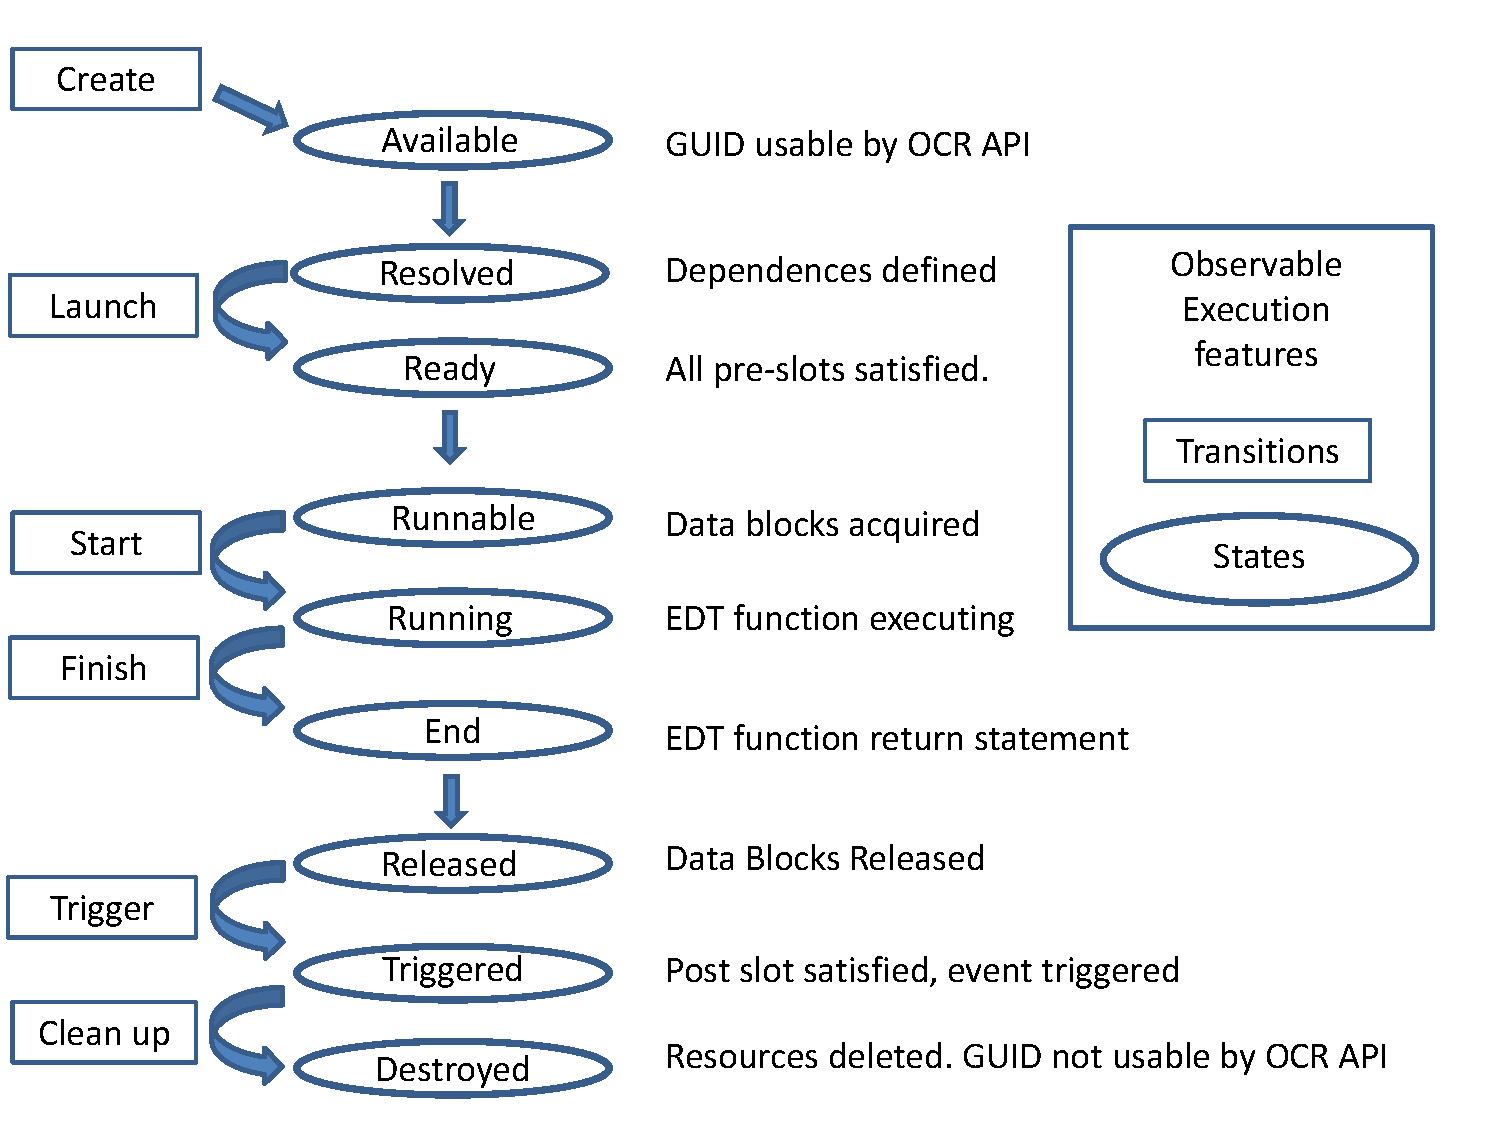
\includegraphics[width=0.9\textwidth]{EDT_exec}
\caption{Observable execution features.}
\label{fig:EDTexec}
\end{figure*}

Normal EDT execution continues until the EDT function returns. The EDT undergoes
a \emph{Finish}\index{EDT transition, finish} transition and the EDT is in
the \emph{End}\index{EDT state, end} state. At some point the EDT will
release the data blocks associated with the EDTs execution and the
EDT enters the \emph{Released}\index{EDT state, released} state.
At this point, any changes made to data blocks will
be available for use by other OCR objects. Later the EDT will
mark its post-slot as satisfied to \emph{Trigger}\index{Trigger} the event
associated with the EDT; thereby becoming a \emph{Triggered} EDT. At
some later point the
system will \emph{Clean-up}\index{EDT transition, clean-up} resources
used by the EDT (including its GUID) and the EDT is destroyed.

Since an EDT is non-blocking, once it
becomes \emph{Runnable} it will run on the OCR platform at some point in the
future. During its run:
\begin{itemize}
\item The EDT can only access data blocks that have been passed in
through its pre-slots as well as any data blocks that the EDT creates
internally. This means that before an EDT starts, the OCR runtime
knows all the data blocks that will be accessed (minus the ones
created within the EDT).

\item The EDT can call into the runtime to create and destroy data
blocks, EDTs and events.

\item The EDT can create \emph{links} between the various OCR
software constructs, termed \emph{dependences}. This is
accomplished through the \code{ocrAddDependence()} function of the OCR
API. The following types of dependences can be created:
\begin{itemize}
\item \emph{Event to Event}: The destination event’s pre-slot is chained
directly to the source event’s post-slot.
For all events but the latch event, this means that the triggering of
the source event will trigger the destination event.

\item \emph{Event to EDT}: One of the destination EDT’s pre-slot is chained
directly to the source event’s post-slot. When the source event is
triggered, this will satisfy the EDT’s pre-slot. If a data block was
associated with the triggering of the source event, that data block
will be made available to the EDT in the dependence array in the
position of the pre-slot. This is a “control + data” dependence. In
the other case, no data block will be made available and the
dependence is akin to a pure control dependence.

\item \emph{Data Block to Event}: Adding a dependence between a data block and an
event is equivalent to satisfying the event with the data block.

\item \emph{Data Block to EDT}: Directly adding a dependence between a data block and
an EDT (a pure data-dependence) immediately satisfies the EDT’s
pre-slot and makes the data block available to the EDT in the
dependence array in the position of the pre-slot.
\end{itemize}

\item The EDT cannot perform any synchronization operations that would
cause it to block inside the body of the task (i.e.\ the EDT must be
non-blocking). The only mechanism for synchronization within OCR is
through the events that link OCR objects, which are explicit to the
runtime.
\end{itemize}

% TODO: Add clarity to the following paragraph on when a programmer
% calls ocrShutdown to terminate even when a few other EDTs haven't
% completed execution, how much is being presumed.

A computation is complete when an EDT terminates the program
(e.g.\ with a call to \code{ocrShutdown()}). Typically, the EDT that
terminates the program is the last EDT in the program DAG, and the
programmer has assured that all other EDTs in the DAG have completed
execution before the function to terminate the program is called.

Since the OCR runtime creates the \code{main()}
function, the programmer does not need to manage the low level
details of initializing and cleanly shutting down OCR.

With both data and tasks conceptually decoupled from their realization
on a computer system, OCR has the flexibility to relocate tasks and data
to respond to failures in the system, achieve a better balance of load
among the processing elements of the computer, or to optimize memory
and energy consumption~\cite{GZCS10,Guo10,CTBCCGYS13,SbBS14}.
This requires that the state of an OCR program can be defined
strictly in terms of which tasks have completed their execution
and the history of updates to data blocks. By saving a log of updates to Data blocks
relative to the tasks that have completed execution, the system can recover
the state of a computation should components of the system fail. This requires,
however, that EDTs execute with transactional semantics.

% This is the end of ch1-exec.tex of the OCR specification.

%
% This is an included file. See the master file for more information.
%

%vivek writes ...
%
%GENERAL COMMENTS:
%
%
%1) A key challenge in defining a memory model is defining the semantics of a data race. All
% memory models usually have the same semantics for data-race-free programs, but vary vastly
% in their definitions of the semantics of data races. For example, I believe that the original
%Release Consistency model had the "memory coherence" assumption which stated that all
% processors see writes to the same location in the same order, which is likely too strong a
%condition for OCR. For a weaker memory model, see Location Consistency (Gao & Sarkar, IEEE ToC 2000).
%

\section{Memory Model}
\index{Memory Model}
\label{sec:MemoryModel}

A memory model defines the values that can be legally observed in
memory when multiple units of execution (e.g.\ processes or threads)
access a shared memory system. The memory model provides programmers
with the tools they need to understand the state of memory, but it
also places restrictions on what a compiler writer can do (e.g.\ which
aggressive optimizations are allowed) and restrictions on what a
hardware designer is allowed to do (e.g.\ the behavior of write
buffers).

To construct a memory model for OCR, we need to present a few
definitions. The operations inside a task execute in a non-blocking
manner. The order of such operations are defined by the
\emph{sequenced-before}\index{sequenced-before} relations defined by
the host C programming language.

When multiple EDTs are running, they execute asynchronously. Usually,
a programmer can make few assumptions about the relative orders of
operations in two different EDTs. At certain points in the execution
of EDTs, however, the OCR program may need to define ordering
constraints. These constraints define
\emph{synchronized-with}\index{synchronized-with} relations.

The ``transitive closure'' of sequenced-before operations inside each
of two EDTs combined with the synchronized-with relations between two
EDTs defines a \emph{happens-before}\index{happens-before}
relationship. For example:
\begin{itemize}
\item if \code{A} is sequenced-before \code{B} in EDT1
\item  if \code{C} is sequenced-before \code{D} in EDT2
\item and  \code{B} is synchronized-with  \code{C} in EDT2
\item then \code{A} happens-before \code{D}.
\end{itemize}
These basic concepts are enough to define the memory model for OCR.


OCR provides a relatively simple memory model. Before an EDT can read
or write a data block, it must first \emph{acquire}\index{Acquire} the data
block. This is not an exclusive relationship by which we mean it is
possible (depending on the mode of the data block in question) for
multiple EDTs to acquire the same data block at the same
time.  When an EDT has finished with a data block and it is ready
to expose any modifications to the data block to other EDTs, it
must \emph{release}\index{Release} that data block.

\begin{quote}
Any function in the OCR runtime that releases a data block must assure
that all loads and stores to the data block occur before the data
block is released and that the release must complete before the
function returns.
\end{quote}

The only way to establish a synchronized-with relation is through the
behavior of events. If the pre-slot of EDT2 is connected to the post-slot
of EDT1, then EDT2 waits for event associated with the post-slot of EDT1 to
trigger. Therefore, the satisfy event from EDT1 synchronizes-with the
triggering of the pre-slot of EDT2. We can establish a happens-before
relationship between the two EDTs if we define the following rule for
OCR.

\begin{quote}
An EDT must complete the release of all of its resources before it
marks its post-event as satisfied.
\end{quote}

An EDT can use data blocks to satisfy events in the body of the task
in addition to the event associated with its post-slot. We can reason
about the behavior of the memory model and establish happens-before
relationship if we define the following rule.

%Vincent's feedback....
%
%"If an EDT uses a Data Block to satisfy an event, all writes to that data block from the EDT must complete
%before the event is triggered.” => I think we already discussed that but I believe you should wait for all the
%db releases that are sequenced-before the satisfy.
%1) This is in case of a db storing guids. db1 has data the edt has written to,  db2 has the guid of db1. %Satisfying ev1 with db2, potentially enables edt2, which spawns edt3 that depends on db1’s guid read from
%db2. With the current rule, db1 may or may not have been released when edt3 acquires it.
%
%db1[0]=1
%db2[0]=db1Guid
%ocrDbRelease(db1)
%ocrDbRelease(db2)
%ocrEventSatisfy(ev1,db2)
%
% TGM responds:
% I submit that since ocrDbRelease(db1) is sequenced before ocrDbRelease(db2) the rules in the memory
%model forces the releases to occur in that order and therefore the model already covers your case.     Can
%you tell me what I'm missing ... because I agree with you completely that the model must force the releases
%to occur in that order prior to the satisfy ... I just think the normal sequenced before relations cover this.
%




\begin{quote}
If an EDT uses a Data Block to satisfy an event, all writes to that data block
from the EDT must complete before the event is triggered.
\end{quote}

Without this rule we can not assume a release operation followed by
satisfying an event defines a sequenced-before relationship that can
be used to establish a happens-before relation.

The core idea in the OCR memory model is that happens-before
relationships are defined in terms of events (the only synchronization
operation in OCR) and the release of OCR objects (such as data
blocks). This is an instance of a \emph{Release
Consistency}\index{Release Consistency} memory model which has the
advantage of being relatively straightforward to apply to OCR
programs.

The safest course for a programmer is to write programs that can be
defined strictly in terms of the release consistency rules. OCR,
however, lets a programmer write programs in which two or more EDTs can
write to a single data block at the same time (or more precisely, the
two EDTs can issue writes in an unordered manner). This may result in a
data race\index{data race} in that the value that is ultimately stored
in memory depends on how a system chooses to schedule operations from
the two EDTs.

Most modern parallel programming languages state that a program that
has a data race\footnote{A \emph{data race} occurs when loads and
stores by two units of execution operate on overlapping memory regions
without a synchronized-with relation to order them} is an illegal
program and the results produced by such a program are undefined.
These programming models then define a complex set of synchronization
constructs and atomic variables so a programmer has the tools needed
to write race-free programs. OCR, however, does not provide any
synchronization constructs beyond the behavior of events. This is not
an oversight. Rather, this restricted synchronization model helps OCR
to better scale on a wider range of parallel computers.

OCR, therefore, allows a programmer to write legal programs that may
potentially contain data races. OCR deals with this situation by
adding two more rules. In both of these rules, we say that address
range $A$ and $B$ are non-overlapping if and only if the set $A_1$ of
8-byte\footnote{The reference to ``8-byte'' words assumes the processing elements
utilize a 64-bit architecture.  For other cases, all references to an 8-byte
word in this specification must be adjusted to match the architecture of the processing elements.}
aligned 8-byte words fully covering $A$ and the set $B_1$ of
8-byte aligned 8-byte words fully covering $B$ do not overlap. For
example, addresses
$0x0$ and $0x7$ overlap (assuming byte level addressing) whereas
$0x0$ and $0x8$ do not.
The first rule deals with the situation of multiple
EDTs writing to a data block with non-overlapping address ranges.
\begin{quote}
If two EDTs write to a single data block without a well defined order,
if the address ranges of the writes do not overlap, the correct result
of each write operation must appear in memory.
\end{quote}

This behavior may seem obvious making it trivial for a system to
support. However, when addresses are distinct but happen to share the
same cache lines or when aggressive optimization of writes occur
through write buffers, an implementation could mask the updates from
one of the EDTs if this rule were not defined in the OCR
specification.

The last rule addresses the case of overlapping address ranges.  Assume that
a system writes values to memory at an atomicity of N-bytes.  This defines
the fundamental store-atomicity for the system\index{store-atomicity}.
\begin{quote}
If two EDTs write to a single data block without a well defined order,
if the address ranges of the writes overlap, the results written to
memory must correspond to one of the legal interleavings of statements
from the two EDTs at an N-byte aligned granularity. Overlapping writes
to non-aligned or smaller than N-byte granularity are not defined.
\end{quote}
For systems that do not provide store-atomicity at any level, N would be 0
and the above rule states that unordered writes to overlapping address
ranges are undefined.
This rule is the well known \emph{sequential consistency}\index{sequential
consistency} rule. It states that the actual result appearing in
memory may be nondeterministic, but it will be well defined and it
will correspond to values from one EDT or the other.

Release consistency remains the safest and best approach to use in
writing OCR programs. It is conceivable that some of the more
difficult rules may be relaxed in future versions of OCR (especially
the sequential consistency rule), but the relaxed consistency model
will almost assuredly always be supported by OCR.

Any memory in OCR that can be accessed by multiple EDTs resides in data blocks.  As
discussed in section~\ref{sec:datablocks} there
are four access modes for the data blocks in OCR. The modes and how they
interact with the OCR memory model are listed as follows.
\begin{itemize}

\item \emph{Read-Write} (default mode)\index{Data Block, read-write}: The EDT may read
and write to the data block.  Multiple EDTs may
write to the same data block at the same time with values constrained according to the
rules in the OCR memory model.

\item \emph{Exclusive write}\index{Data Block, exclusive write}: The
EDT requires that it is the only EDT that can commit write operations to a data block at a
given time.  Writes must follow a sequential total order; i.e.\ when more than one EDT is writing
to a data block in exclusive write mode, all the writes from one EDT must complete before
a subsequent EDT can acquire and then write to the data block.  This serializes the execution of
EDTs that acquire data blocks in exclusive write mode.

\item \emph{Read only}\index{Data Block, read only}: The EDT
will only read from the Data Block. The OCR Runtime does
not restrict the ability of other EDTs to write to the data block.  The
visibility of those writes are undefined; i.e.\ an implementation may
choose whether or not to make writes by other EDTs visible.

\item \emph{Constant}\index{Data Block,constant}: The EDT will only read from the
data block and the OCR runtime will assure that once the data block is acquired,
writes from other EDTs will not be visible.

\end{itemize}


% This is the end of ch1-memory.tex of the OCR specification.
%%%%%
\section{Organization of this document}
\label{sec:Organization of this document}
% Vivek writes ... Add a new section on OCR semantics that covers properties such as
% deadlock, data races, functional determinism, and structural determinism.
%
%  TGM responds ... I am confused by what you are asking for.  This is a specfication.
%  Do these concepts really belong here?

The remainder of this document is structured as follows:

\begin{itemize}
\item Chapter~\ref{chap:OCRAPI} defines the OCR Application Programming Interface.

\item Appendix~\ref{chap:Appendix A} contains a set of pedagogical examples.

\item Appendix~\ref{chap:Appendix B} contains a set of proposed OCR Extensions.

\item Appendix~\ref{chap:Appendix C} contains notes specific to current implementations of OCR.

\item Appendix~\ref{chap:Appendix D} documents the ``change history''
  for OCR and this specification.
\end{itemize}


% This is the end of ch1-main.tex of the OCR specification.
